\documentclass{article}

\usepackage{booktabs,multirow,tabularx,tikz,amssymb,amsmath}
\usetikzlibrary{bpmn}

\title{The Tikz BPMN package}
\author{Sander J.J. Leemans}

\begin{document}
	\maketitle
	
	This manual describes the BPMN Tikz package, used to draw BPMN models.
	
	\def\event#1{
		\eventsymbol{#1}
		&
		\eventcode{#1}
	}
	
	\def\eventsymbol#1{
		\begin{tikzpicture}[baseline]
			\node [#1] {};
		\end{tikzpicture}
	}
	\def\eventcode#1{
		\texttt{\textbackslash{}node [#1] \{\};}
	}
	
	\def\boundary#1{
		\begin{tikzpicture}[baseline]
			\node [task, label={[#1]225:}] {};
		\end{tikzpicture}
		&
		\texttt{\textbackslash{}node [task, label=\{[#1]225:\}] \{\};}
	}
	
	\section{Usage}
		Place the file \texttt{tikzlibrarybpmn.code.tex} in the same folder as your .tex file, and include \verb!\usetikzlibrary{bpmn}! in the preamble of your .text file.
		
		\subsection{Gateways}
			\begin{tabularx}{\linewidth}{cX}
				\toprule
				Symbol & code\\
				\midrule
				\event{exclusive gateway}\newline\eventcode{xor gateway}\\
				\event{parallel gateway}\newline\eventcode{and gateway}\\
				\event{inclusive gateway}\newline\eventcode{or gateway}\\
				\event{eventbased gateway}\\
				\bottomrule
			\end{tabularx}
		
		\subsection{Events}
			\begin{tabularx}{\linewidth}{cX}
				\toprule
				Symbol & code\\
				\midrule
				\event{start event}\\
				\event{end event}\\
				\midrule
				\event{message start event}\\
				\event{catching message intermediate event}\\
				\event{throwing message intermediate event}\\
				\event{message end event}\\
				\midrule
				\event{timer start event}\\
				\eventsymbol{timer event}
				&
				\texttt{\textbackslash{}node [timer event] \{\};}\newline
				\texttt{\textbackslash{}node [intermediate timer event] \{\};}
				\\
				\midrule
				\event{throwing compensation intermediate event}\\
				\event{throwing compensation end event}\\
				\midrule
				\eventsymbol{error event} & \eventcode{error event} \newline \eventcode{throwing error end event}\\
				\midrule
				\event{signal start event}\\
				\event{catching signal intermediate event} \newline \eventcode{signal intermediate event}\\
				\event{throwing signal intermediate event}\\
				\event{signal end event}\\
				\bottomrule
			\end{tabularx}
		
		\subsubsection{Background colour}
			The background colour is an optional argument for several event styles, and required to be set if the background is not white for correct rendering.
			The default can be set using 
			\verb=\colorlet{defaultbackgroundcolour}{new default colour}= after loading the package.
			
		\subsection{Tasks \& sub-processes}
			\begin{tabularx}{\linewidth}{cX}
				\toprule
				Symbol & code\\
				\midrule
					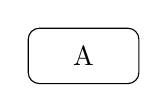
\begin{tikzpicture}[baseline]
						\node [task] {A};
					\end{tikzpicture}
					&
					\texttt{\textbackslash{}node [task] \{A\};}
				\\
					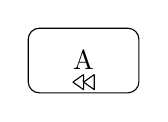
\begin{tikzpicture}[baseline]
						\node [compensation task] {A};
					\end{tikzpicture}
					&
					\texttt{\textbackslash{}node [compensation task] \{A\};}
				\\
					\begin{tikzpicture}[baseline]
						\node [loop task] {A};
					\end{tikzpicture}
					&
					\texttt{\textbackslash{}node [loop task] \{A\};} \newline
					requires the \texttt{amssymb} and \texttt{amsmath} packages
				\\
					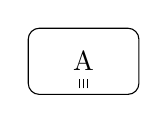
\begin{tikzpicture}[baseline]
						\node [multiinstance task] {A};
					\end{tikzpicture}
					&
					\texttt{\textbackslash{}node [multiinstance task] \{A\};}
				\\
				
				\midrule
				
				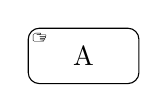
\begin{tikzpicture}[baseline]
					\node [manual task] {A};
				\end{tikzpicture}
				&
				\texttt{\textbackslash{}node [manual task] \{A\};}
				\\
				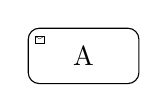
\begin{tikzpicture}[baseline]
					\node [receive task] {A};
				\end{tikzpicture}
				&
				\texttt{\textbackslash{}node [receive task] \{A\};}
				\\
				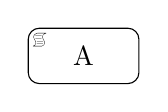
\begin{tikzpicture}[baseline]
					\node [script task] {A};
				\end{tikzpicture}
				&
				\texttt{\textbackslash{}node [script task] \{A\};}
				\\
				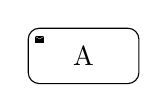
\begin{tikzpicture}[baseline]
					\node [send task] {A};
				\end{tikzpicture}
				&
				\texttt{\textbackslash{}node [send task] \{A\};}
				\\
				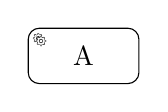
\begin{tikzpicture}[baseline]
					\node [service task] {A};
				\end{tikzpicture}
				&
				\texttt{\textbackslash{}node [service task] \{A\};}
				\\
				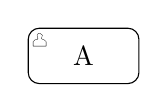
\begin{tikzpicture}[baseline]
					\node [user task] {A};
				\end{tikzpicture}
				&
				\texttt{\textbackslash{}node [user task] \{A\};}
				\\
				\bottomrule
			\end{tabularx}
				
			\begin{tabularx}{\linewidth}{cX}
				\toprule
				Symbol & code\\
				\midrule
					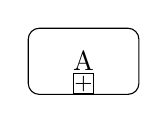
\begin{tikzpicture}[baseline]
						\node [subprocess] {A};
					\end{tikzpicture}
					&
					\texttt{\textbackslash{}node [subprocess] \{A\};} \newline
					\texttt{\textbackslash{}node [collapsed subprocess] \{A\};}
				\\
					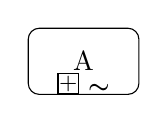
\begin{tikzpicture}[baseline]
						\node [adhoc subprocess] {A};
					\end{tikzpicture}
					&
					\texttt{\textbackslash{}node [adhoc subprocess] \{A\};} \newline
					\texttt{\textbackslash{}node [collapsed adhoc subprocess] \{A\};}
				\\
					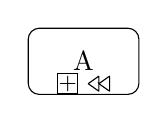
\begin{tikzpicture}[baseline]
						\node [compensation subprocess] {A};
					\end{tikzpicture}
					&
					\texttt{\textbackslash{}node [compensation subprocess] \{A\};} \newline
					\texttt{\textbackslash{}node [collapsed compensation subprocess] \{A\};}
				\\
					\begin{tikzpicture}[baseline]
						\node [loop subprocess] {A};
					\end{tikzpicture}
					&
					\texttt{\textbackslash{}node [loop subprocess] \{A\};} \newline
					\texttt{\textbackslash{}node [collapsed loop subprocess] \{A\};} \newline
					requires the \texttt{amssymb} and \texttt{amsmath} packages
				\\
					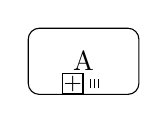
\begin{tikzpicture}[baseline]
						\node [multiinstance subprocess] {A};
					\end{tikzpicture}
					&
					\texttt{\textbackslash{}node [multiinstance subprocess] \{A\};} \newline
					\texttt{\textbackslash{}node [collapsed multiinstance subprocess] \{A\};}
				\\
				
				\midrule
				
					\multirow{2}{*}{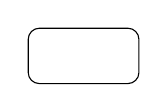
\begin{tikzpicture}[baseline]
						\node [expanded subprocess] {};
					\end{tikzpicture}}
					&
					\texttt{\textbackslash{}node [expanded subprocess] \{\};}\newline
					use in combination with the \verb=fit= key
				\\
					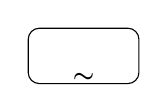
\begin{tikzpicture}[baseline]
						\node [expanded adhoc subprocess] {};
					\end{tikzpicture}
					&
					\texttt{\textbackslash{}node [expanded adhoc subprocess] \{\};}\newline
					use in combination with the \verb=fit= key
				\\
					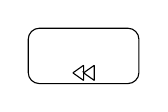
\begin{tikzpicture}[baseline]
						\node [expanded compensation subprocess] {};
					\end{tikzpicture}
					&
					\texttt{\textbackslash{}node [expanded compensation subprocess] \{\};}\newline
					use in combination with the \verb=fit= key
				\\
					\begin{tikzpicture}[baseline]
						\node [expanded loop subprocess] {};
					\end{tikzpicture}
					&
					\texttt{\textbackslash{}node [expanded loop subprocess] \{\};}\newline
					use in combination with the \verb=fit= key
				\\
					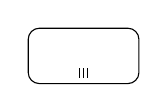
\begin{tikzpicture}[baseline]
						\node [expanded multiinstance subprocess] {};
					\end{tikzpicture}
					&
					\texttt{\textbackslash{}node [expanded multiinstance subprocess] \{\};}\newline
					use in combination with the \verb=fit= key
				\\
					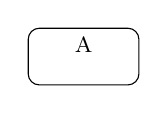
\begin{tikzpicture}[baseline]
						\node [subprocess label=A] {};
					\end{tikzpicture}
					&
					\texttt{\textbackslash{}node [subprocess label=A] \{\};}\newline
					use in combination with the \verb=fit= key
				\\
				\bottomrule
			\end{tabularx}
			
		\subsection{Event sub-processes}
			\begin{tabularx}{\linewidth}{cX}
				\toprule
				Symbol & code\\
				\midrule
				\event{message subprocess event}\\
				\event{timer subprocess event}\\
				\event{signal subprocess event}\\
				\event{compensation subprocess event}\\
				\event{error subprocess event}\\
				\midrule
				\event{message noninterrupting subprocess event}\\
				\event{timer noninterrupting subprocess event}\\
				\event{signal noninterrupting subprocess event}\\
				\midrule
				\event{message event subprocess}\\
				\event{timer event subprocess}\\
				\event{signal event subprocess}\\
				\event{compensation event subprocess}\\
				\event{error event subprocess}\\
				\midrule
				\event{message noninterrupting event subprocess}\\
				\event{timer noninterrupting event subprocess}\\
				\event{signal noninterrupting event subprocess}\\
				\bottomrule
			\end{tabularx}
			
		\subsection{Boundary events}
			In the following, the number 225 controls the position of the boundary event (in degrees).
			Naturally, a label can be used on any node.
			To connect associations to a label, use the style \texttt{name=}.
			
			\noindent\begin{tabularx}{\linewidth}{cX}
				\toprule
				Symbol & code\\
				\midrule
				\boundary{timer boundary event}\\
				\boundary{message boundary event}\\
				\boundary{signal boundary event}\\
				\boundary{compensation boundary event}\\
				\boundary{error boundary event}\\
				\boundary{timer noninterrupting boundary event}\\
				\boundary{message noninterrupting boundary event}\\
				\boundary{signal noninterrupting boundary event}\\
				\bottomrule
			\end{tabularx}
			
			All boundary events use fill to draw over the border of the parent node, and accept an argument for the fill colour.
			The default fill colour can be changed using \verb=\colorlet{defaultbackgroundcolour}{new default colour}= after loading the package.
			
		\subsection{Data}
			\begin{tabularx}{\linewidth}{cX}
				\toprule
				Symbol & code\\
				\midrule
				\event{data object}\\
				\event{data collection}\\
				\event{data store}\\
				\bottomrule
			\end{tabularx}
			
		
		\subsection{Resources}
			\begin{tabularx}{\linewidth}{cX}
				\toprule
				Symbol & code\\
				\midrule
					\begin{tikzpicture}[baseline]
						\node [pool] {\phantom{ABCDEF}\strut};
					\end{tikzpicture}
					&
					\texttt{\textbackslash{}node [pool] \{\};} \newline
					use in combination with the \verb=fit= key
				\\
					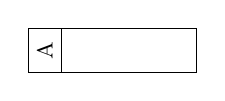
\begin{tikzpicture}[baseline]
						\node [pool label=A] {\phantom{ABCDEF}\strut};
					\end{tikzpicture}
					&
					\texttt{\textbackslash{}node [pool label=A] \{\};} \newline
					use in combination with the \verb=fit= key
				\\
				\bottomrule
			\end{tabularx}
			
\end{document}